% --------------------------------------------------------------
% This is all preamble stuff that you don't have to worry about.
% Head down to where it says "Start here"
% --------------------------------------------------------------
 
\documentclass[12pt]{article}\usepackage[]{graphicx}\usepackage[]{color}
%% maxwidth is the original width if it is less than linewidth
%% otherwise use linewidth (to make sure the graphics do not exceed the margin)
\makeatletter
\def\maxwidth{ %
  \ifdim\Gin@nat@width>\linewidth
    \linewidth
  \else
    \Gin@nat@width
  \fi
}
\makeatother

\definecolor{fgcolor}{rgb}{0.345, 0.345, 0.345}
\newcommand{\hlnum}[1]{\textcolor[rgb]{0.686,0.059,0.569}{#1}}%
\newcommand{\hlstr}[1]{\textcolor[rgb]{0.192,0.494,0.8}{#1}}%
\newcommand{\hlcom}[1]{\textcolor[rgb]{0.678,0.584,0.686}{\textit{#1}}}%
\newcommand{\hlopt}[1]{\textcolor[rgb]{0,0,0}{#1}}%
\newcommand{\hlstd}[1]{\textcolor[rgb]{0.345,0.345,0.345}{#1}}%
\newcommand{\hlkwa}[1]{\textcolor[rgb]{0.161,0.373,0.58}{\textbf{#1}}}%
\newcommand{\hlkwb}[1]{\textcolor[rgb]{0.69,0.353,0.396}{#1}}%
\newcommand{\hlkwc}[1]{\textcolor[rgb]{0.333,0.667,0.333}{#1}}%
\newcommand{\hlkwd}[1]{\textcolor[rgb]{0.737,0.353,0.396}{\textbf{#1}}}%

\usepackage{framed}
\makeatletter
\newenvironment{kframe}{%
 \def\at@end@of@kframe{}%
 \ifinner\ifhmode%
  \def\at@end@of@kframe{\end{minipage}}%
  \begin{minipage}{\columnwidth}%
 \fi\fi%
 \def\FrameCommand##1{\hskip\@totalleftmargin \hskip-\fboxsep
 \colorbox{shadecolor}{##1}\hskip-\fboxsep
     % There is no \\@totalrightmargin, so:
     \hskip-\linewidth \hskip-\@totalleftmargin \hskip\columnwidth}%
 \MakeFramed {\advance\hsize-\width
   \@totalleftmargin\z@ \linewidth\hsize
   \@setminipage}}%
 {\par\unskip\endMakeFramed%
 \at@end@of@kframe}
\makeatother

\definecolor{shadecolor}{rgb}{.97, .97, .97}
\definecolor{messagecolor}{rgb}{0, 0, 0}
\definecolor{warningcolor}{rgb}{1, 0, 1}
\definecolor{errorcolor}{rgb}{1, 0, 0}
\newenvironment{knitrout}{}{} % an empty environment to be redefined in TeX

\usepackage{alltt}
 
\usepackage[margin=1in]{geometry} 
\usepackage{amsmath,amsthm,amssymb}
 \usepackage{amsfonts}
\newcommand{\N}{\mathbb{N}}
\newcommand{\Z}{\mathbb{Z}}
 
\newenvironment{theorem}[2][Theorem]{\begin{trivlist}
\item[\hskip \labelsep {\bfseries #1}\hskip \labelsep {\bfseries #2.}]}{\end{trivlist}}
\newenvironment{lemma}[2][Lemma]{\begin{trivlist}
\item[\hskip \labelsep {\bfseries #1}\hskip \labelsep {\bfseries #2.}]}{\end{trivlist}}
\newenvironment{exercise}[2][Exercise]{\begin{trivlist}
\item[\hskip \labelsep {\bfseries #1}\hskip \labelsep {\bfseries #2.}]}{\end{trivlist}}
\newenvironment{problem}[2][Problem]{\begin{trivlist}
\item[\hskip \labelsep {\bfseries #1}\hskip \labelsep {\bfseries #2.}]}{\end{trivlist}}
\newenvironment{question}[2][Question]{\begin{trivlist}
\item[\hskip \labelsep {\bfseries #1}\hskip \labelsep {\bfseries #2.}]}{\end{trivlist}}
\newenvironment{corollary}[2][Corollary]{\begin{trivlist}
\item[\hskip \labelsep {\bfseries #1}\hskip \labelsep {\bfseries #2.}]}{\end{trivlist}}
\newenvironment{BaseCase}[2][Base Case]{\begin{trivlist}
\item[\hskip \labelsep {\bfseries #1}\hskip \labelsep {\bfseries #2.}]}{\end{trivlist}}
\newenvironment{Answer}[2][Answer]{\begin{trivlist}
\item[\hskip \labelsep {\bfseries #1}\hskip \labelsep {\bfseries #2.}]}{\end{trivlist}}
\newenvironment{Sketch}[2][Sketch]{\begin{trivlist}
\item[\hskip \labelsep {\bfseries #1}\hskip \labelsep {\bfseries #2.}]}{\end{trivlist}}
\IfFileExists{upquote.sty}{\usepackage{upquote}}{}
\begin{document}
 
% --------------------------------------------------------------
%                         Start here
% --------------------------------------------------------------
 
\title{Homework 2\\
$t$ Tests}%replace X with the appropriate number
\author{Steve Bronder\\ %replace with your name
Statistical Inference} %if necessary, replace with your course title
 
\maketitle
 
\begin{exercise}{1}Find a dataset and perform a t-test to evaluate whether the mean number of days below 32 degrees for the six weeks after Punxsutawney Phil sees his shadow is greater than or equal to the mean number of days below 32 degrees for the six weeks after Phil does not see his shadow.
\end{exercise}

\section*{Answer}

To evaluate whether Punxsutawney Phil can accurately predict six more weeks of winter we have to define a criteria for evaluation. Our criteria will be whether or not Phil accurately predicted a greater than average number of days with temperature below 32 degrees for the months of February and March of each year. If Phil predicts a long winter for a year we will give him 1 point out of a possible 65 points. Phil is limited to 65 points because our data ranges from 1950 to 2014 $(T=65)$. We gather data from the National Climate Data Center\footnote{http://www.ncdc.noaa.gov/cdo-web/datatools/findstation} for the county Punxsutawney Phil is located in, Jefferson County, PA. To find whether Phil saw his shadow we gather data from stormfax\footnote{http://www.stormfax.com/ghogday.htm} on whether or not he saw his shadow for our target years. \\

 Our data set is comprised of three variables, The year, the number of days it is below 32 degrees in the months of February and March, and whether or not Phil saw his shadow for a given year. Lets have a look at our data. We remove the years in which a moving average was used to gain the number of days for unreported periods. We then plot the data using 
 
\begin{knitrout}
\definecolor{shadecolor}{rgb}{0.969, 0.969, 0.969}\color{fgcolor}\begin{kframe}
\begin{alltt}
\hlcom{# Read in csv}
\hlstd{Ghog}\hlkwb{<-}\hlkwd{read.csv}\hlstd{(}\hlstr{"./ghog_clean.csv"}\hlstd{,}\hlkwc{header}\hlstd{=}\hlnum{TRUE}\hlstd{)}

\hlcom{# Remove moving average years}
\hlstd{Ghog2} \hlkwb{<-} \hlstd{Ghog[}\hlkwd{c}\hlstd{(}\hlnum{1}\hlopt{:}\hlnum{47}\hlstd{,}\hlnum{53}\hlopt{:}\hlnum{65}\hlstd{),]}

\hlkwd{attach}\hlstd{(Ghog2)}

\hlkwd{plot}\hlstd{(Year,daysbelow32 )}

\hlcom{# No shadow line and shadow line in graph}
\hlkwd{abline}\hlstd{(}\hlkwd{mean}\hlstd{(daysbelow32[ghog}\hlopt{==}\hlstr{"NOShadow"}\hlstd{]),}\hlnum{0}\hlstd{,}\hlkwc{col}\hlstd{=}\hlstr{"red"}\hlstd{)}
\hlkwd{abline}\hlstd{(}\hlkwd{mean}\hlstd{(daysbelow32[ghog}\hlopt{==}\hlstr{"Shadow"}\hlstd{]),}\hlnum{0}\hlstd{)}

\hlcom{# make color points}
\hlkwd{points}\hlstd{(Year[ghog}\hlopt{==}\hlstr{"NOShadow"}\hlstd{],daysbelow32[ghog}\hlopt{==}\hlstr{"NOShadow"}\hlstd{],}\hlkwc{col}\hlstd{=}\hlstr{"red"}\hlstd{,}\hlkwc{pch}\hlstd{=}\hlnum{4}\hlstd{)}
\end{alltt}
\end{kframe}
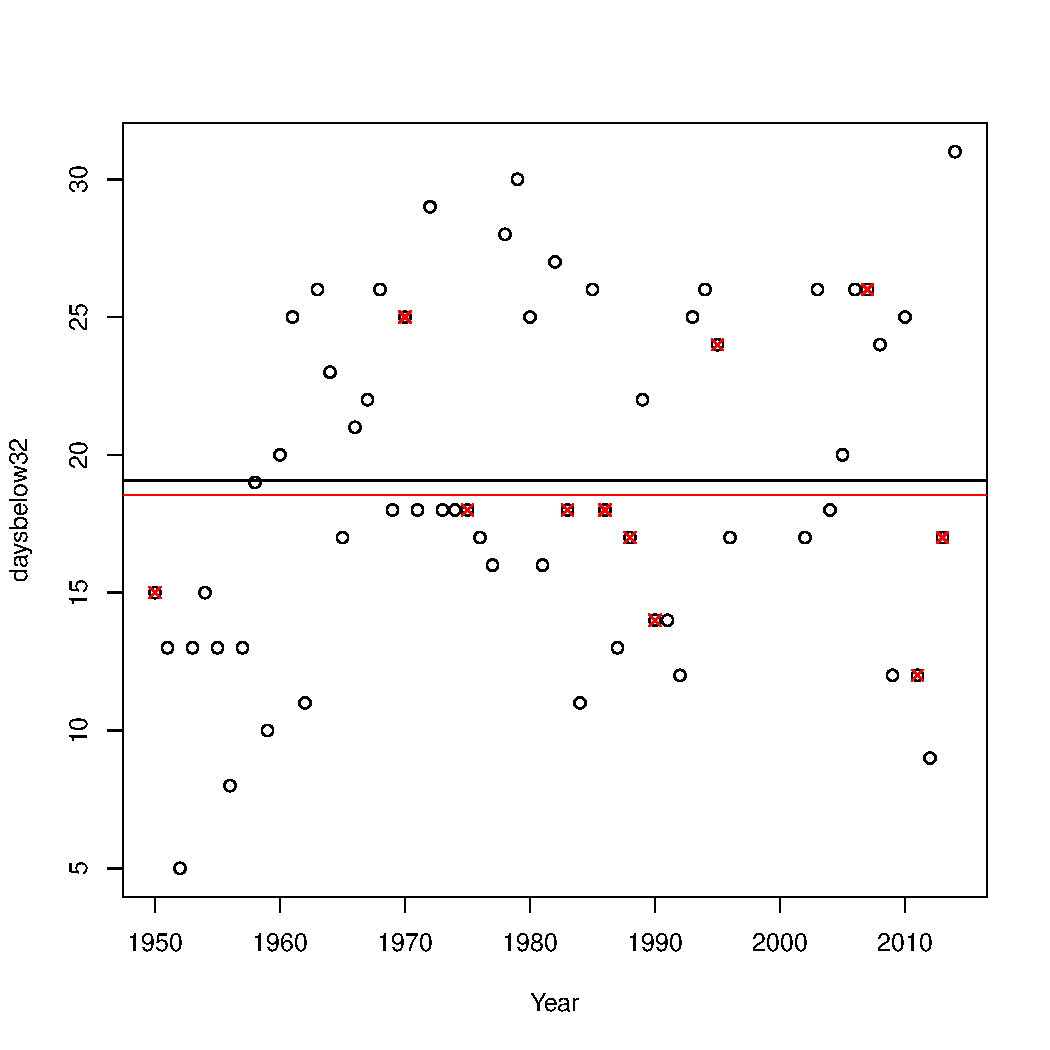
\includegraphics[width=\maxwidth]{figure/manipulation-1} 
\begin{kframe}\begin{alltt}
\hlstd{mean.b32.ns} \hlkwb{<-} \hlkwd{mean}\hlstd{(daysbelow32[ghog}\hlopt{==}\hlstr{"NOShadow"}\hlstd{])}
\hlstd{mean.b32.s} \hlkwb{<-} \hlkwd{mean}\hlstd{(daysbelow32[ghog}\hlopt{==}\hlstr{"Shadow"}\hlstd{])}
\hlstd{sd.b32.ns} \hlkwb{<-} \hlkwd{sd}\hlstd{(daysbelow32[ghog}\hlopt{==}\hlstr{"NOShadow"}\hlstd{])}
\hlstd{sd.b32.s} \hlkwb{<-} \hlkwd{sd}\hlstd{(daysbelow32[ghog}\hlopt{==}\hlstr{"Shadow"}\hlstd{])}
\hlstd{ln.b32.ns} \hlkwb{<-} \hlkwd{length}\hlstd{(daysbelow32[ghog}\hlopt{==}\hlstr{"NOShadow"}\hlstd{])}
\hlstd{ln.b32.s} \hlkwb{<-} \hlkwd{length}\hlstd{(daysbelow32[ghog}\hlopt{==}\hlstr{"Shadow"}\hlstd{])}
\end{alltt}
\end{kframe}
\end{knitrout}

At this point we run a two sample t-test by collecting the mean, standard deviation, and length of the days the temperature was below 32 degrees catagorized by whether or not the almighty groundhog saw his shadow.

\begin{knitrout}
\definecolor{shadecolor}{rgb}{0.969, 0.969, 0.969}\color{fgcolor}\begin{kframe}
\begin{alltt}
\hlstd{ttest.s} \hlkwb{<-} \hlstd{(mean.b32.ns}\hlopt{-}\hlstd{mean.b32.s)}\hlopt{/}\hlkwd{sqrt}\hlstd{((sd.b32.ns}\hlopt{^}\hlnum{2}\hlopt{/}\hlstd{ln.b32.ns)} \hlopt{+}
                                           \hlstd{(sd.b32.s}\hlopt{^}\hlnum{2}\hlopt{/}\hlstd{ln.b32.s))}

\hlstd{ttest.s}
\end{alltt}
\begin{verbatim}
## [1] -0.3112187
\end{verbatim}
\begin{alltt}
\hlcom{#t test with alternative greater}
\hlkwd{t.test}\hlstd{(daysbelow32[ghog}\hlopt{==}\hlstr{"NOShadow"}\hlstd{],daysbelow32[ghog}\hlopt{==}\hlstr{"Shadow"}\hlstd{],}
       \hlkwc{alternative}\hlstd{=}\hlkwd{c}\hlstd{(}\hlstr{"greater"}\hlstd{))}
\end{alltt}
\begin{verbatim}
## 
## 	Welch Two Sample t-test
## 
## data:  daysbelow32[ghog == "NOShadow"] and daysbelow32[ghog == "Shadow"]
## t = -0.3112, df = 20.111, p-value = 0.6206
## alternative hypothesis: true difference in means is greater than 0
## 95 percent confidence interval:
##  -3.373306       Inf
## sample estimates:
## mean of x mean of y 
##  18.54545  19.06122
\end{verbatim}
\begin{alltt}
\hlcom{#t test with alternative not equal}
\hlkwd{t.test}\hlstd{(daysbelow32[ghog}\hlopt{==}\hlstr{"NOShadow"}\hlstd{],daysbelow32[ghog}\hlopt{==}\hlstr{"Shadow"}\hlstd{],}
       \hlkwc{alternative}\hlstd{=}\hlkwd{c}\hlstd{(}\hlstr{"two.sided"}\hlstd{))}
\end{alltt}
\begin{verbatim}
## 
## 	Welch Two Sample t-test
## 
## data:  daysbelow32[ghog == "NOShadow"] and daysbelow32[ghog == "Shadow"]
## t = -0.3112, df = 20.111, p-value = 0.7588
## alternative hypothesis: true difference in means is not equal to 0
## 95 percent confidence interval:
##  -3.971524  2.939984
## sample estimates:
## mean of x mean of y 
##  18.54545  19.06122
\end{verbatim}
\begin{alltt}
\hlkwd{pt}\hlstd{(}\hlopt{-}\hlnum{.3112}\hlstd{,}\hlnum{20.11}\hlstd{)}
\end{alltt}
\begin{verbatim}
## [1] 0.3794258
\end{verbatim}
\end{kframe}
\end{knitrout}

With a p-value of .62 for the alternative of greather than and a p-value of .76 for the alternative of equal our results imply that the difference in mean number of days below 32 when the groundhog does not see his shadow is statistically insignificant from the number of days below 32 degrees for the day he sees his shadow. A t-test is only valid if the data we have is approximately distributed normally. As such we generate histograms and smoothed density plots of the days below 32 degrees catagorized by whether the all knowing groundhog saw his shadow. We then create a pretty graph using ggplot2 and the wesanderson package. This step is crucial as everyone loves a pretty graph.

\begin{knitrout}
\definecolor{shadecolor}{rgb}{0.969, 0.969, 0.969}\color{fgcolor}\begin{kframe}
\begin{alltt}
\hlcom{#Histograms to check normality}
\hlkwd{par}\hlstd{(}\hlkwc{mfrow}\hlstd{=}\hlkwd{c}\hlstd{(}\hlnum{2}\hlstd{,}\hlnum{2}\hlstd{))}
\hlkwd{hist}\hlstd{(daysbelow32[ghog}\hlopt{==}\hlstr{"NOShadow"}\hlstd{],}\hlkwc{nclass}\hlstd{=}\hlnum{8}\hlstd{,}\hlkwc{main}\hlstd{=}\hlstr{"Historgram of No Shadow"}\hlstd{)}
\hlkwd{hist}\hlstd{(daysbelow32[ghog}\hlopt{==}\hlstr{"Shadow"}\hlstd{],}\hlkwc{nclass}\hlstd{=}\hlnum{8}\hlstd{,}\hlkwc{main}\hlstd{=}\hlstr{"Historgram of Shadow"}\hlstd{)}

\hlcom{#Density plot to check normality}
\hlkwd{plot}\hlstd{(}\hlkwd{density}\hlstd{(daysbelow32[ghog}\hlopt{==}\hlstr{"NOShadow"}\hlstd{],}\hlkwc{adjust}\hlstd{=}\hlnum{1.5}\hlstd{),}\hlkwc{main}\hlstd{=}\hlstr{"Density of No Shadow"}\hlstd{)}
\hlkwd{plot}\hlstd{(}\hlkwd{density}\hlstd{(daysbelow32[ghog}\hlopt{==}\hlstr{"Shadow"}\hlstd{],}\hlkwc{adjust}\hlstd{=}\hlnum{1.5}\hlstd{),}\hlkwc{main}\hlstd{=}\hlstr{"Density of Shadow"}\hlstd{)}
\end{alltt}
\end{kframe}
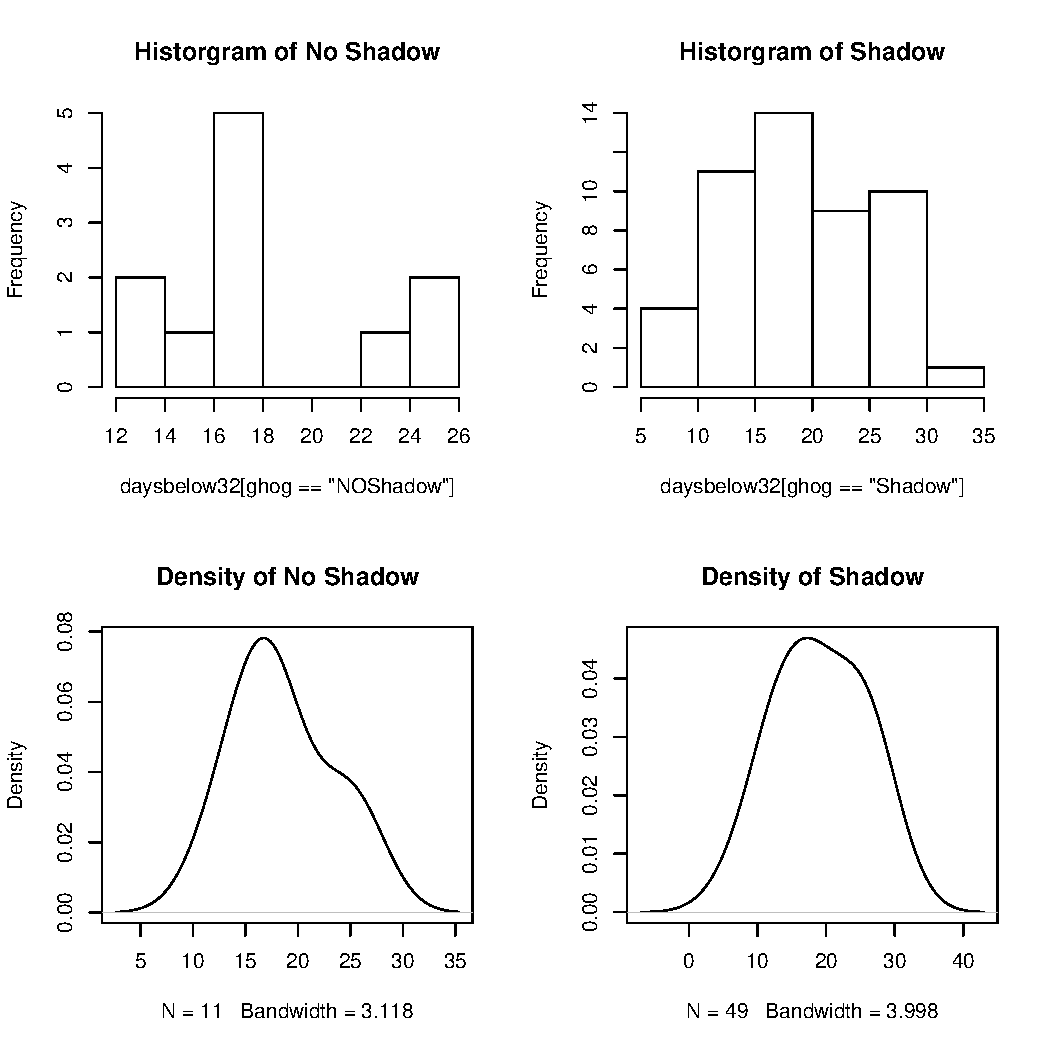
\includegraphics[width=\maxwidth]{figure/plots-1} 
\begin{kframe}\begin{alltt}
\hlcom{# Pretty ggplot to check normality}

\hlkwd{library}\hlstd{(ggplot2)}
\hlkwd{library}\hlstd{(wesanderson)}

\hlstd{pretty} \hlkwb{<-} \hlkwd{ggplot}\hlstd{(Ghog2,}\hlkwd{aes}\hlstd{(}\hlkwc{colour}\hlstd{=ghog))}\hlopt{+}
  \hlkwd{scale_color_manual}\hlstd{(}\hlkwc{values} \hlstd{=} \hlkwd{wes.palette}\hlstd{(}\hlnum{2}\hlstd{,} \hlstr{"Royal1"}\hlstd{))}\hlopt{+}
  \hlkwd{geom_density}\hlstd{(}\hlkwd{aes}\hlstd{(}\hlkwc{x}\hlstd{=daysbelow32),}\hlkwc{adjust}\hlstd{=}\hlnum{1.5}\hlstd{,,}\hlkwc{size}\hlstd{=}\hlnum{1.5} \hlstd{)}  \hlopt{+}
  \hlkwd{ggtitle}\hlstd{(}\hlstr{"Density of Number of Days Below 32"}\hlstd{)}\hlopt{+}
    \hlkwd{theme}\hlstd{(}\hlkwc{axis.title.x} \hlstd{=} \hlkwd{element_blank}\hlstd{(),} \hlkwc{axis.title.y} \hlstd{=} \hlkwd{element_blank}\hlstd{())}\hlopt{+}
   \hlkwd{theme}\hlstd{(}\hlkwc{plot.title} \hlstd{=} \hlkwd{element_text}\hlstd{(}\hlkwc{size} \hlstd{=} \hlkwd{rel}\hlstd{(}\hlnum{1.8}\hlstd{)))} \hlopt{+} \hlkwd{xlim}\hlstd{(}\hlnum{0}\hlstd{,}\hlnum{40}\hlstd{)}
\hlstd{pretty}
\end{alltt}
\end{kframe}
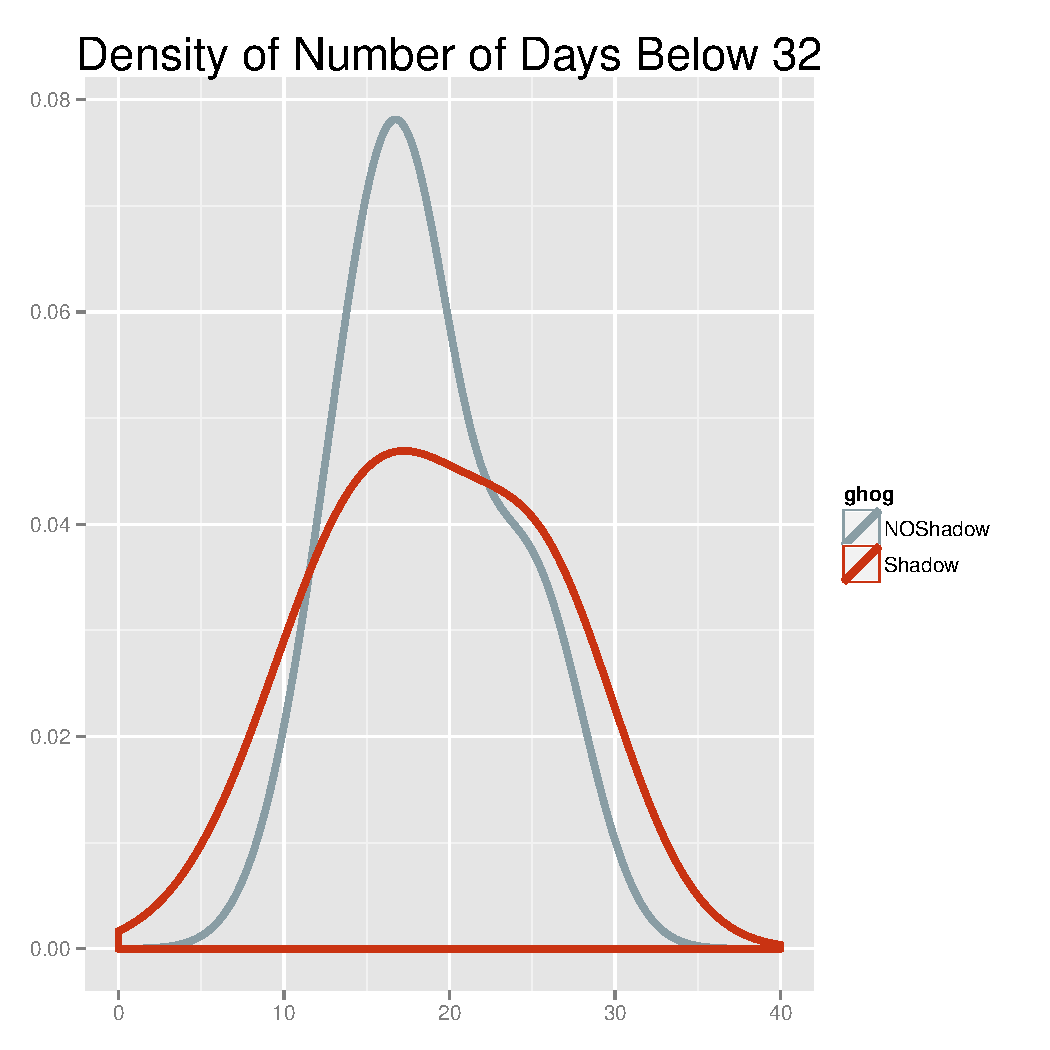
\includegraphics[width=\maxwidth]{figure/plots-2} 

\end{knitrout}

In conclusion, with our plots showing an approximately normal distribution for our rather small samples, we conclude the t-test is valid. Our results imply that the difference in mean number of days below 32 degrees when the groundhog does not see his shadow is statistically insignificant from the number of days below 32 degrees for the day he sees his shadow. 
%HOMEWORK 
% 1. Apply a two-sample t-test to your groundhog data.
% 2, Check normality assumption
% 3. State Appropriate null and alternative hypothesis
% 4. Compute test statistics df and p-value using t-test
% 5. Provide an in-context conclusion in plain language



 
 
% --------------------------------------------------------------
%     You don't have to mess with anything below this line.
% --------------------------------------------------------------
 
\end{document}
